In this chapter basic music theory necessary for the understanding of the report is presented.
\\ \\
An example of a staff system with 15 notes is shown in figure \ref{fig:cmajor}. A note in such a system is generally a symbolic representation of a certain tone, which is associated to a particular frequency (specified in hertz, Hz). Each note thus contains information about the frequency of the associated tone and also about its duration in time. A note sheet is therefore actually a symbolic representation of a diagram over time and frequency, which is also called a spectrogram.

\begin{figure}[H]
    \centering
    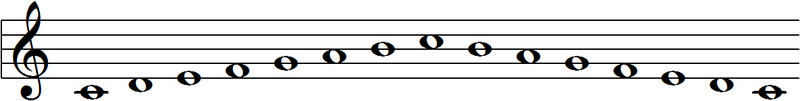
\includegraphics[width = 0.6\textwidth]{figures/Cmajor.png}
    \caption{Example of notes in a staff system.}
    \label{fig:cmajor}
\end{figure}

\noindent
A staff system consists of 5 horizontal lines whereupon the notes are placed. Basically, only 12 key notes are repeated throughout the system but each with different frequencies. The key notes with the same names differ by an interval of $n$ octaves for some integer $n$ and are said to be octave equivalent. \cite{MusicTheory} The relation in frequency between two tones $A_0$ and $A_n$ are thus $A_n = 2^n A_0, n \in \mathbb{Z}$, and $A_n$ is therefore $n$ octaves above $A_0$.
\\ \\
The notes in the staff system are named by the letters $A$-$G$ depending on their vertical position. After $G$ the naming is repeated with the next $A$, which lies an octave above the previous one. Furthermore, between several of these tones lie semitones, which are noted as e.g. $A$\hashsharp{}. Table \ref{tab:freq} shows all tones in the interval $A_3$-$A_4$.
\\ \\
To be able to distinguish between octave equivalent tones they are e.g. noted as $A_4$ and $A_5$. $A_4$ is also called the concert pitch and is normally chosen to be $440$ Hz by definition but may vary by $\pm 3$ Hz depending on who's playing. All other tones are set relative to the chosen frequency of $A_4$ since it is the $12^{th}$ key note after $A_3$, whose frequency is half the size of $A_4$'s. The relation in frequency between two neighbouring tones, e.g. $A$ and $A$\hashsharp, is therefore $A$\hashsharp \ $= \sqrt[\leftroot{-2}\uproot{2}12]{2} \cdot A$. \cite{MusicTheory} The frequencies of the tones in the interval $A_3$-$A_4$ rounded off to the nearest integer is shown in table \ref{tab:freq}.
\\ \\
When a tone is played the tone's overtones will sound along with the actual tone. The frequency of a tone's overtone is an integer multiple of the original tone's frequency, and this phenomena is therefore typically reflected through the octave equivalent tones of the original one. However, the tone $A_2$ with frequency $110$ Hz also has the overtone $E_3$ ($330$ Hz) along with the octave equivalent tones $A_3$ ($220$ Hz), $A_4$ ($440$ Hz) and $A_5$ ($880$ Hz). If several instruments play at the same time all the original tones and overtones are mixed, which is one of several reasons why it is difficult to automatically translate music played by several instruments into a single note sheet. On the other hand, if only one instrument is playing, the overtones are not mixed together, and the tone is thus easily distinguished from the overtones since the tone in question then usually will be the one with the lowest frequency. The overtones therefore complicate the determination of the original tone, but the determination is not impossible if the tone e.g. is played alone in an anechoic room. This is shown in figure (insert reference to figure below). Playing a pitch alone in an anechoic room is a way of minimizing noise factors which is further described in chapter (insert reference to the proper chapter).

\begin{table}[H]
\centering
\caption{Frequencies of the pitches $A_3$-$A_4$ shown in Hz and rounded off to nearest integer.}
\label{tab:freq}
\begin{tabular}{|l|c|c|c|c|c|c|c|c|c|c|c|c|c|}
\hline
Pitch & $A_3$ & $A_3$\hashsharp & $B_3$ & $C_3$ & $C_3$\hashsharp & $D_3$ & $D_3$\hashsharp & $E_3$ & $F_3$ & $F_3$\hashsharp & $G_3$ & $G_3$\hashsharp & $A_4$ \\ \hline
Freq & 220 & 233 & 247 & 262 & 277 & 294 & 311 & 330 & 349 & 370 & 392 & 415 & 440 \\ \hline
\end{tabular}
\end{table}

\noindent
*Insert spectogram showing a single pitch with overtones here.*

\section{Sound}
Sound is often perceived as waves moving through air with a constant velocity relative to the surrounding material. A music instrument playing a certain tone makes the surrounding particles oscillate with a certain frequency, and the neighbouring particles are set in motion as well with the same frequency. The frequency is specified in hertz which is the number of cycles per second. Therefore, e.g. $440$ Hz corresponds to $440$ oscillations every second.
\\ \\
Among others, a musical tone is often characterized by its pitch and intensity. The pitch is determined by the frequency, and the intensity is determined by their amplitude which is the size of the oscillations. Naturally, the intensity decreases over distance because the energy from the instrument needs to be distributed over more particles. But the frequency remains the same - that is, if the musician is able to maintain the exact same pitch which is difficult on most instruments.
\\ \\
This project is delimited to deal with a guitar as the musical instrument. A guitar is a string instrument with usually 6 strings from the so-called sadle over the sound hole and fretboard to the machine head which may be turned to tune the guitar. The fretboard of the guitar consists of frets which are approximately one semitone apart, and they are thus pressed down while bringing the string in motion with the other hand to create different tones. Eventually, the sound is amplified by the soundboard and the body, and the sound comes out of the sound hole.
\\ \\
The pitch of the tone being played is determined by the lenght, mass and tension of the strings. The lenght of the strings is the only variable while playing on a guitar, and in general, cutting the lenght of the string in half doubles the frequency. \cite{WikiGuitar} \cite{AcousticGuitar} 


%Dansk tekst
%I dette kapitel introduceres grundlæggende musikteori, der er nødvendig for forståelsen af projektet.
%\\ \\
%I nodesystemet er en node en symbolsk repræsentation af en bestemt tone, som er tilknyttet en specifik frekvens (angivet i hertz, Hz). Hver node indeholder således information om tonens højde og desuden også om dens varighed. Et nodeark er således en symbolsk repræsentation af et diagram over tid og frekvens, hvilket også kaldes et spektrogram.
%\\ \\
%Til at notere noder benytter man et nodesystem, der består af fem vandrette linjer, hvor noderne er placeret. Grundlæggende findes der 12 forskellige toner, som gentages igennem nodesystemet. Principielt set findes der således flere toner med samme navn men med forskellige frekvenser, og disse toner siges at være oktavækvivalente, da den ene ligger et antal oktaver over den anden. Forholdet i frekvens mellem 2 oktavækvivalente toner $A_0$ og $A_n$ er derfor $A_n = 2^n A_0, n \in \mathbb{Z}$, og $A_n$ er således $n$ oktaver over $A_0$.
%\\ \\
%Noderne i nodesystemet består først og fremmest af stamtoner, som navngives med bogstaverne $A$-$G$ afhængigt af deres vertikale placering. Efter $G$ starter navngivningen forfra med det næste $A$, der ligger en oktav over det forrige. Mellem flere af stamtonerne ligger desuden andre toner, som sammen med stamtonerne udgør de 12 grundtoner. Afstanden mellem alle grundtonerne er en halv tone, og tonen mellem $C$ og $D$ noteres som C\hashsharp{}.
%\\ \\
%For at skelne mellem de oktavækvivalente toner noteres de for eksempel som $A_4$ og $A_5$. $A_4$ kaldes også kammertonen og vælges per definition normalt til at være $440$ Hz, men kan dog afvige med $\pm 3$ Hz afhængigt af den enkelte musiker eller orkester, der spiller musikken. Alle andre toner kan defineres ud fra den valgte frekvens for $A_4$, da $A_4$ er den 12. grundtone efter $A_3$, som har halvt så stor frekvens som $A_4$. Forholdet i frekvens mellem to naboliggende toner, for eksempel $C$ og $C$\hashsharp, er således $C$\hashsharp \ $= \sqrt[\leftroot{-2}\uproot{2}12]{2} \cdot C$. \cite{MusicTheory} Ud fra dette forhold ses det, at tonesystemet bygger på en logaritmisk skala. Frekvenserne for tonerne $A_3$-$A_4$ afrundet til nærmeste heltal er vist i tabel \ref{frektoner}.
%\\ \\
%Når en tone spilles vil tonens overtoner klinge sammen med den pågældende tone. En tones overtone er et heltals-multiplum af den oprindelige tone, og dette fænomen kommer således blandt andet til udtryk for de oktavækvivalente toner af den oprindelige tone. Hvis flere instrumenter spiller sammen blandes overtonerne sammen, hvilket er en vigtig årsag til, at det er problematisk at oversætte optaget musik spillet af flere instrumenter til noder. Hvis kun ét instrument spiller blandes overtonerne derimod ikke sammen, og så vil den spillede tone som udgangspunkt være tonen med den laveste frekvens. Overtonerne komplicerer derfor bestemmelsen af tonen, men det er ikke umuligt, hvis tonen spilles alene i for eksempel et lyddødt rum. Dette fænomen ses på spektogrammet i figur (indsæt reference).
%\\ \\ \\ \\
%\begin{table}[H]
%\centering
%\caption{Frekvensen for tonerne $A_3$-$A_4$ afrundet til nærmeste heltal.}
%\label{frektoner}
%\begin{tabular}{|l|c|c|c|c|c|c|c|c|c|c|c|c|c|}
%\hline
%Tone & $A_3$ & $A_3$\hashsharp & $B_3$ & $C_3$ & $C_3$\hashsharp & $D_3$ & $D_3$\hashsharp & $E_3$ & $F_3$\hashsharp & $F_3$ & $G_3$ & $G_3$\hashsharp & $A_4$ \\ \hline
%Frekvens & 220 & 233 & 247 & 262 & 277 & 294 & 311 & 330 & 349 & 370 & 392 & 415 & 440 \\ \hline
%\end{tabular}
%\end{table}
%
%
%
%
%
%
%*Indsæt spektogram af en enkelt spillet tone med tilhørende overtone her.*